\documentclass{standalone}

\usepackage{tikz}
\usetikzlibrary{arrows.meta}


\begin{document}

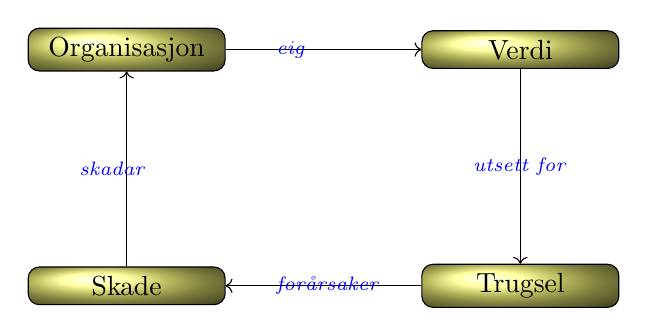
\begin{tikzpicture}
  \tikzstyle{term}=[minimum width=25mm,rounded corners,draw,ball color=yellow!50]
  \tikzstyle{lab}=[rounded corners,font=\scriptsize\itshape,text=blue]
  \node [term] (asset) at (5,3) {Verdi} ;
  \node [term] (org) at (0,3) {Organisasjon} ;
  \node [term] (threat) at (5,0) {Trugsel} ;
  \node [term] (impact) at (0,0) {Skade} ;
  \path [->,draw] (org) edge node[lab] {\parbox{12mm}{eig}} (asset) ;
  \path [->,draw] (asset) edge node[lab] {\parbox{12mm}{utsett for}} (threat) ;
   \path [->,draw] (threat) edge node[lab] {\parbox{12mm}{forårsaker}} (impact) ;
  \path [->,draw] (impact) edge node[lab] {\parbox{12mm}{skadar}} (org) ;
\end{tikzpicture}
\end{document}
